\documentclass[a4paper, 12pt, oneside]{scrartcl}

\usepackage[a4paper, total={7in, 10in}]{geometry}
\usepackage[utf8]{inputenc}          
\usepackage[T2A]{fontenc}            
\usepackage[english, russian]{babel} 
\usepackage{amsmath}
\usepackage{graphicx}
\usepackage[top=1cm]{geometry}


\renewcommand{\baselinestretch}{1.5}

\newcommand\tab[1][1cm]{\hspace*{#1}}

\begin{document}
	\begin{center}
	{\scshape\Large\bfseries Дальневосточный федеральный университет \par}
	{\scshape\Large Школа естественных наук \par}
	{\large Лабораторная работа №3 по дифференциальным уравнениям \par}
	{\large\bfseries Потоцкая Анастасия Б8203а \par}
	\end{center}
	\newcommand{\ud}{\mathrm{d}}
	В лабораторной работе использовалась система компьютерной алгебры wxMaxima. 
		\begin{enumerate}

		\item[1.] 
		% Найдите общее решение системы
		% исследуйте на устойчивость нулевое решение
% нарисуйте фазовый портрет в окрестности нуля
		\begin{equation*}
		  	\begin{cases}
   				\dot{x} = x + y \\
   				\dot{y	} = -2x + 3y 
		  	\end{cases}
		  	\tab
			\begin{cases}
				\dot{x} = -11x - 8y \\
				\dot{y} = 8x + 5y
			\end{cases}

		\end{equation*}

		\textbf{Тип: }
		Однородная система линейных  дифференциальных уравнений с постоянными коэффициентам \\
	
		\textbf{Общее решение: }

		\begin{equation*}
			\begin{cases}
			x(t)=e^{2t}( \frac{\sin(t)}{2}(3y(0)-2x(0)) + x(0)\cos(t)) \\
			y(t)=e^{2t}( \frac{\sin(t)}{2}(2y(0)-4x(0)) + y(0)\cos(t))

			\end{cases}
		\end{equation*}

		\begin{equation*}
			\begin{cases}
			x(t)=-8y(0)te^{-3t}-8x(0)te^{-3t}+x(0)e^{-3t} \\
			y(t)=8y(0)te^{-3t}+8x(0)te^{-3t}+y(0)e^{-3t}

			\end{cases}
		\end{equation*}
		
		\textbf{Исследуем на устойчивость нулевое решение: } \\
		Корни характеристического уравнения первой системы:\\
		$\lambda_{1,2}=2\pm\imath $\\
		Решение неусточиво. \\ 
		Корни характеристического уравнения второй системы:\\
		$\lambda_{1,2} = {-3, 2}$\\
		Решение неусточиво.
		
		\textbf{Фазовый портрет в окрестности нуля: }
	\begin{figure}[h]
		\centering
		\begin{tabular}{cc}
		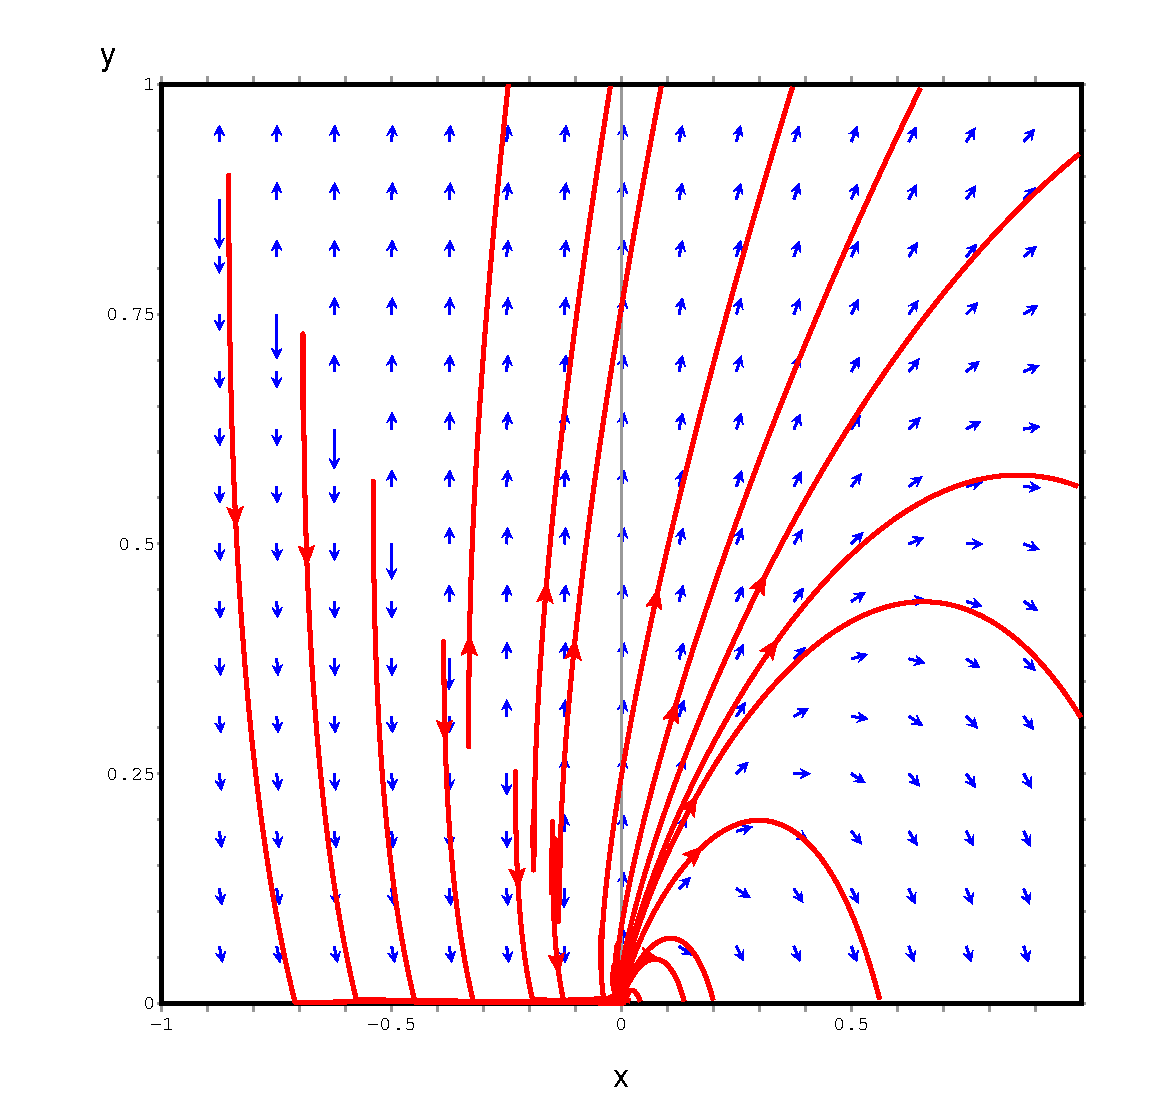
\includegraphics[width=0.3\linewidth]{p1}
		&
		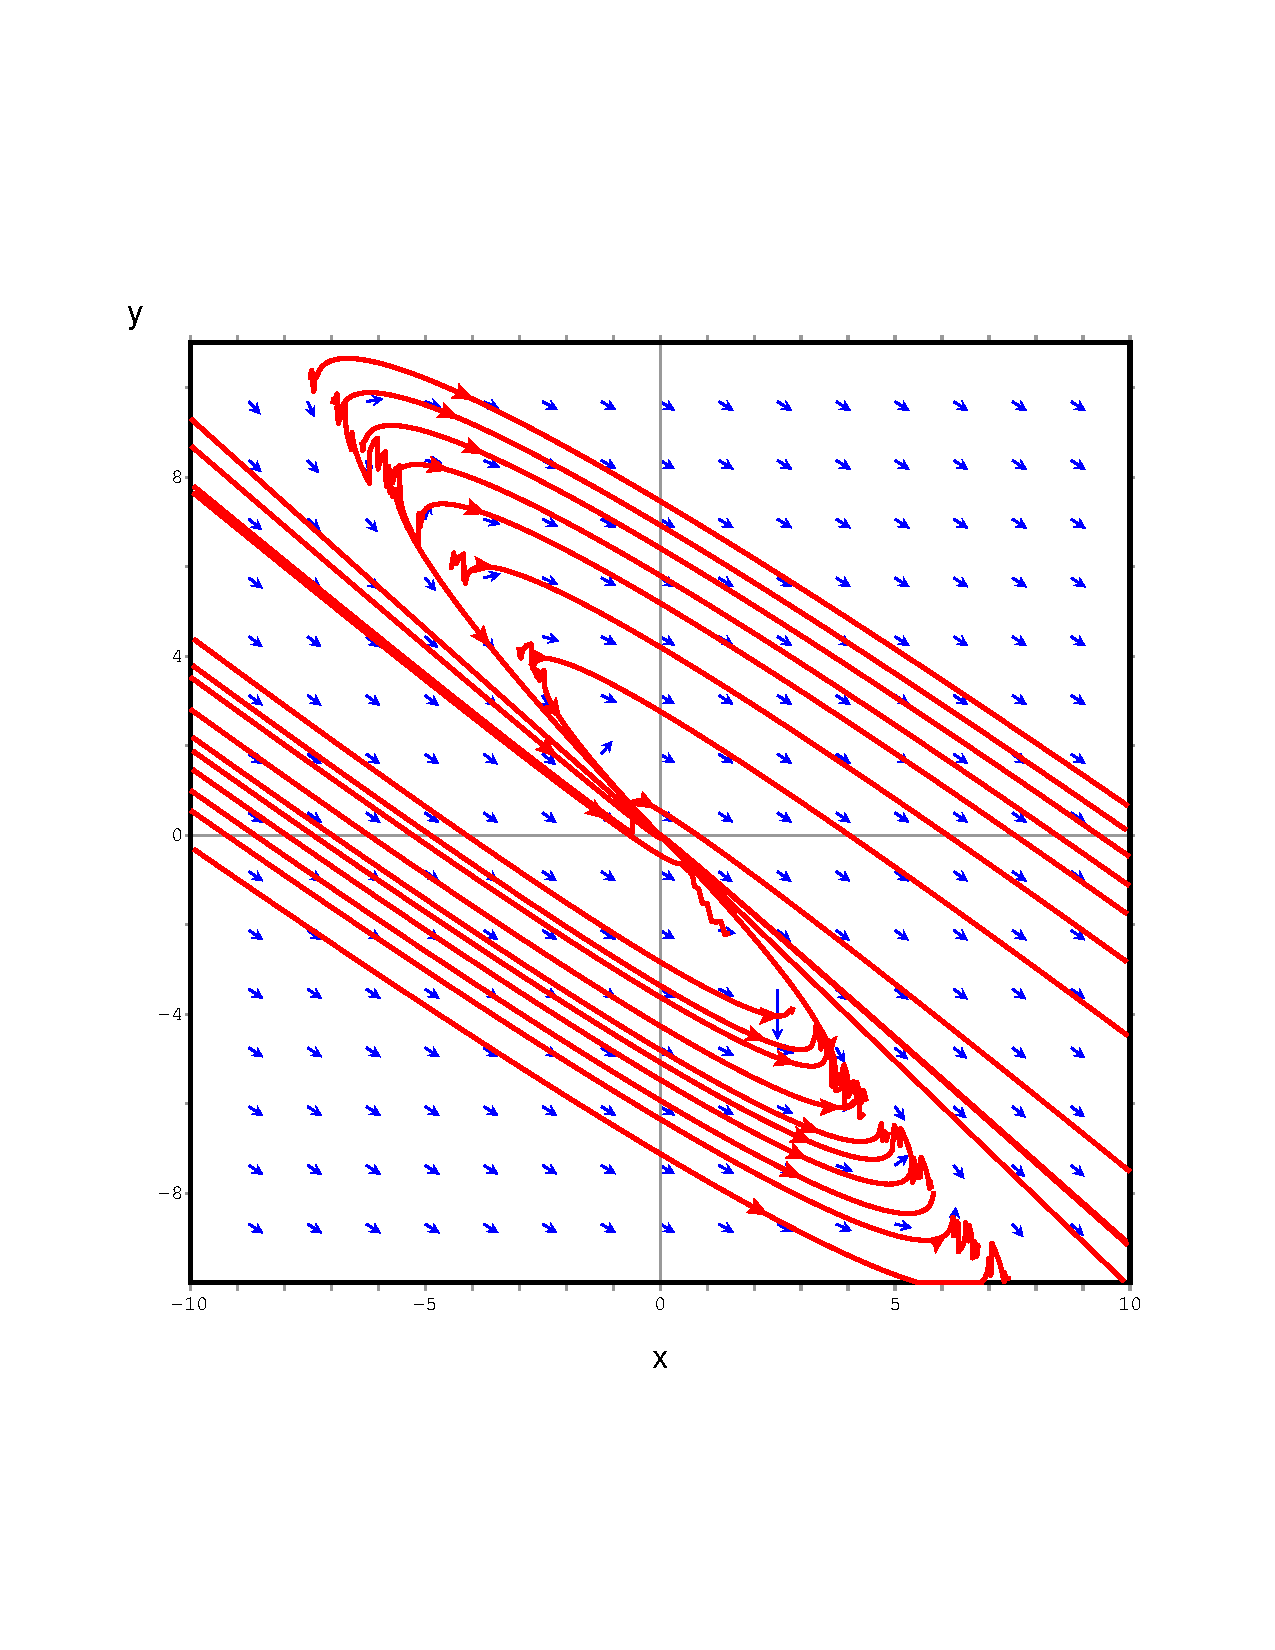
\includegraphics[width=0.3\linewidth]{p2}
		\end{tabular}
		\caption{Фазовые портреты}
		\label{fig:mpr}
	\end{figure}
		
		\pagebreak

		\textbf{Команды вводимые в wxMaxima: }
		\begin{verbatim}
		eqn_1:'diff(x(t), t) = x(t) + y(t);
		eqn_2:'diff(y(t), t) = -2*x(t) + 3*y(t);
		desolve([eqn_1, eqn_2], [x(t), y(t)]);

		eqn_1:'diff(x(t),t)=-11*x(t)-8*y(t);
		eqn_2:'diff(y(t),t)=8*x(t)+5*y(t);
		desolve([eqn_1,eqn_2],[x(t),y(t)]);
	
		plotdf((-2*x + 3*y)/(x + y), [x, -1, 1], [y, 0, 1]);
		plotdf((8*x + 5*y)/(-11*x - 8*y), [x, -10, 10], [y, -10, 11]);
		\end{verbatim} 
		
		\item[2.]
	% Решите задачу Коши и исследуйте решение на устойчивость
		
		\begin{equation*}
			\begin{cases}
			\dot{x}= x + y\\
			\dot{y}= 3x - y

			\tab 
			x(0) = 0, y(0) = -4
			\end{cases}
		\end{equation*}


		\textbf{Тип:}
		 Однородная система линейных  дифференциальных уравнений с постоянными коэффициентам  \\
	
		\textbf{Частное решение: }

		\begin{equation*}
			\begin{cases}
			x(t)=-3e^{2t}-e^{-2t} \\
			y(t)=3e^{-2t}-3e^{2t} 
			\end{cases}
		\end{equation*}

		
		\textbf{Исследуем на устойчивость нулевое решение: } \\
		Корни характеристического уравнения:\\
		$\lambda_{1,2}= {-2, 2}$\\
		Решение неусточиво. \\ 
		
		\textbf{Команды вводимые в wxMaxima: }
		\begin{verbatim}
	a: matrix([1,1],[3,-1]);
	eigenvalues(a);
	
	de1:'diff(x(t),t)=x(t)+y(t);
	de2:'diff(y(t),t)=3*x(t)-y(t);
	atvalue(y(t),t=0,0);
	atvalue(x(t),t=0,-4);
	desolve([de1,de2],[y(t),x(t)]);
	\end{verbatim}


		\item[3.]
		
		\begin{equation*}
			\begin{cases}
			\dot{x}=  x - 7y\\
			\dot{y}= x + 9y + t

			\end{cases}
		\end{equation*}


		\textbf{Тип:  }
	Неоднородная система линейных  дифференциальных уравнений с постоянными коэффициентам \\
		\textbf{Общее решение: }

		\begin{equation*}
			\begin{cases}
			x(t)=-\frac{e^{8t}}{384}(448y(0)+64x(0)+7)+\frac{e^{2t}}{24}(28y(0)+28x(0)+7)-\frac{7t}{16}-\frac{35}{128} \\
			y(t)=\frac{e^{8t}}{384}(448y(0)+64x(0)+7)-\frac{e^{2t}}{24}(4y(0)+4x(0)+1)-\frac{t}{16}+\frac{3}{128} 
			\end{cases}
		\end{equation*} 
		
		\textbf{Команды вводимые в wxMaxima: }
		\begin{verbatim}
	de1:'diff(x(t),t)=x(t)-7*y(t);
	de2:'diff(y(t),t)=x(t) + 9 * y(t) + t;
	desolve([de1,de2],[y(t),x(t)]);
	\end{verbatim}
		
		\item[4.]

\begin{equation*}
		  	\begin{cases}
   				\dot{x} = x + 9y + 8z \\
   				\dot{y} = 2y + 3z \\
   				\dot{z} = 6z
		  	\end{cases}
		  	\tab \begin{cases}
				\dot{x} = x - 9y - 3z \\
				\dot{y} = 3x + 4y + 9z \\
				\dot{z} = 3x + 7z + 6z 
			\end{cases}
			\tab \begin{cases}
				\dot{x} = x + y + 4z \\
				\dot{y} = 2x - y + 2z \\
				\dot{z} = 4x - 6y + z 
			\end{cases}

		\end{equation*}

		\textbf{Тип:}
		Однородная система линейных  дифференциальных уравнений с постоянными коэффициентам  \\
	
		\textbf{Общее решение первой системы: }
		\begin{equation*}
			\begin{cases}
			x(t)=\frac{59}{20}z(0)e^{6t}-\frac{e^{2t}}{4}(27z(0)-36y(0))+\frac{e^{t}}{5}(19z(0)-45y(0)+5x(0)) \\
			y(t)=\frac{3}{4}z(0)e^{6t}-\frac{e^{2t}}{4}(3z(0)-4y(0)) \\
			z(t)=z(0)e^{6t}
			\end{cases}
		\end{equation*}

		\textbf{Общее решение второй системы: }
		\begin{equation*}
			\begin{cases}
			x(t)=-30z(0)te^{7t}+18y(0)te^{7t}-6x(0)te^{7t}+(9z(0)-9y(0)+ x(0))e^{7t} +
			\nonumber \\ \quad \quad +(9y(0)-9z(0))e^{4t}
			\\
			y(t)=15z(0)te^{7t}-9y(0)te^{7t}+3x(0)te^{7t}+(3y(0)-2z(0))e^{7t}+
			\nonumber \\ \quad \quad +(2z(0)-2y(0))e^{4t}
			\\
			z(t)=15z(0)te^{7t}-9y(0)te^{7t}+3x(0)te^{7t}+
			\nonumber \\ \quad \quad + (3y(0)-2z(0))e^{7t}+(3z(0)-3y(0))e^{4t}
			\end{cases}
		\end{equation*}		

		\textbf{Общее решение третьей системы: }
		\begin{equation*}
			\begin{cases}
			
			x(t)=e^{2t}(\frac{\sin(t)}{2}(\frac{(2(31z(0)-85y(0)+31x(0)))}{26}+\frac{(4(3z(0)+14y(0)+3x(0)))}{26}) +
			\nonumber\\ \quad \quad + \frac{((3z(0)+14y(0)+3x(0))\cos(t))}{13})- \frac{e^{-3t}}{13}(3z(0)+14y(0)-10x(0))

			\\
			y(t)=e^{2t}(\frac{\sin(t)}{2}(4z(0)-6y(0)+4x(0))+y(0)\cos(t))
			\\
			z(t)=e^{2t}((\frac{4}{26}(10z(0)-14y(0)+10x(0))-\frac{2}{26}(18z(0)-20y(0)+18x(0)))\frac{\sin(t)}{2} + 
			\nonumber\\ \quad \quad	+\frac{\cos(t)}{13}(10z(0)-14y(0)+10x(0))+ 
			+\frac{e^{-3t}}{13}(3z(0)+14y(0)-10x(0))
			

			\end{cases}
		\end{equation*}
		
		\textbf{Исследуем на устойчивость нулевое решение: } \\
		Корни характеристического уравнения первой системы:\\
		$\lambda_{1,2,3} = {1, 2, 6}$\\
		Решение неусточиво. \\ 
		Корни характеристического уравнения второй системы:\\
		$\lambda_{1,2,3} = {7, 7, 4}$\\
		Решение неусточиво. \\
		Корни характеристического уравнения третьей системы:\\
		$\lambda_{1,2,3} = {-3, 2\pm\imath}$\\
		Решение неусточиво. \\
		
		\textbf{Команды вводимые в wxMaxima: }
		\begin{verbatim}
	a: matrix([1,9,8],[0,2,3],[0,0,6]);
	eigenvalues(a);
	
	a: matrix([1,-9,-3],[3,4,9],[3,0,13]);
	eigenvalues(a);
	
	a: matrix([1,1,4],[2,-1,2],[4,-6,1]);
	eigenvalues(a);
   				
	de1:'diff(x(t),t)=x(t) + 9*y(t) + 8*z(t);
	de2:'diff(y(t),t)=2*y(t)+3*z(t);
	de3:'diff(z(t),t)=6*z(t);
	desolve([de1,de2,de3],[x(t),y(t),z(t)]);
	
	
	de1:'diff(x(t),t)=x(t)-9*y(t)-3*z(t);
	de2:'diff(y(t),t)=3*x(t)+4*y(t)+9*z(t);
	de3:'diff(z(t),t)=3*x(t)+13*z(t);
	desolve([de1,de2,de3],[x(t),y(t),z(t)]);
	
	de1:'diff(x(t),t)=x(t)+y(t)+4*z(t);
	de2:'diff(y(t),t)=2*x(t)-y(t)+2*z(t);
	de3:'diff(z(t),t)=4*x(t)-6*y(t)+z(t);
	desolve([de1,de2,de3],[x(t),y(t),z(t)]);
		\end{verbatim} 

		\item[5.]
	
	\begin{equation*}
	\begin{cases}
	\dot{x}=3x-4y-6z+13t^2 - 12t + 36
	\\
	\dot{y}=2x-6y-2z+6t^2-6t+24
	\\
	\dot{z}=x+6y-4z+3t^2-4t+6
	\end{cases}
	\tab
	\begin{cases}
	\dot{x}=3x-8y-3z+35e^{2t}
	\\
	\dot{y}=-9x-y-9z+51e^{2t}
	\\
	\dot{z}=-4x + 8y+2z-20e^{2t}
	\end{cases}
	\end{equation*}
	\textbf{Тип:}
	 Неоднородная система линейных  дифференциальных уравнений с постоянными коэффициентам  \\
	
	\textbf{Общее решение: }
	\begin{equation*}
	\begin{cases}
	x(t)=e^{-2t}(\frac{\sin(2t)}{4}(-16z(0)-16y(0)+16x(0)+180) + 
	\nonumber\\ \quad \quad  +(2z(0)+8y(0)-2x(0)-25)\cos(2t))-
	\nonumber\\ \quad \quad  -(6z(0)+24y(0)-9x(0)-106)\frac{e^{-3t}}{3}+3t^2+2t-\frac{31}{3}
\\
	y(t)=e^{-2t}\frac{\sin(2t)}{4}*(-4z(0)-8y(0)+4x(0)+46)+\frac{\cos(2t)}{2}(2y(0)-1))+
	\nonumber\\ \quad \quad+t^2+\frac{1}{2}
	\\
	z(t)=e^{-2t}(\frac{\sin(2t)}{4}(-8z(0)-4y(0)+8x(0)+30)+
	\nonumber\\ \quad \quad +\frac{\cos(2t)}{2}(6z(0)+16y(0)-6x(0)-71))-
	\nonumber\\ \quad \quad - \frac{e^{-3t}}{3}(6z(0)+24y(0)-9x(0)-106)+3t^2-2t+\frac{1}{6}
	\end{cases}
	\end{equation*}
	
	\begin{equation*}
	\begin{cases}
	x(t)=\frac{e^{6t}}{49}(51z(0)-56y(0)+100x(0)-94)-e^{2t} -
	\nonumber\\ \quad \quad -72z(0)t\frac{e^{-t}}{7}-72x(0)t\frac{e^{-t}}{7}+
	\nonumber\\ \quad \quad  +360t\frac{e^{-t}}{7}-\frac{e^{-t}}{49}(51z(0)-56y(0)+51x(0)-143)
	\\
	y(t)=2e^{2t}-9e^{-t}z(0)t*-9e^{-t}x(0)t+45e^{-t}t+e^{-t}(y(0)-2)
	\\
	z(t)=-\frac{e^{6t}}{49}(51z(0)-56y(0)+100x(0)-94)+
	\nonumber\\ \quad \quad +6e^{2t}+72z(0)t\frac{(e^{-t}}{7}+72x(0)t\frac{e^{-t}}{7}-360t\frac{e^{-t}}{7}+\frac{e^{-t}}{49}(100z(0)-56y(0)+100x(0)-388)
	\end{cases}
	\end{equation*}	
		
	\textbf{Команды вводимые в wxMaxima: }
		\begin{verbatim}
		de1:'diff(x(t),t)=3*x(t)-4*y(t)-6*z(t)+13*t^2-12*t+36;
		de2:'diff(y(t),t)=2*x(t)-6*y(t)-2*z(t)+6*t^2-6*t+24;
		de3:'diff(z(t),t)=x(t)+6*y(t)-4*z(t)+3*t^2-4*t+6;
		desolve([de1,de2,de3],[x(t),y(t),z(t)]);
		
		de1:'diff(x(t),t)=3*x(t)-8*y(t)-3*z(t)+35*exp(2*t);
		de2:'diff(y(t),t)=-9*x(t)-y(t)-9*z(t)+51*exp(2*t);
		de3:'diff(z(t),t)=-4*x(t)+8*y(t)+2*z(t)-20*exp(		de1:'diff(x(t),t)=3*x(t)-8*y(t)-3*z(t)+35*exp(2*t);
		de2:'diff(y(t),t)=-9*x(t)-y(t)-9*z(t)+51*exp(2*t);
		de3:'diff(z(t),t)=-4*x(t)+8*y(t)+2*z(t)-20*exp(2*t);
		desolve([de1,de2,de3],[x(t),y(t),z(t)]);2*t);
		desolve([de1,de2,de3],[x(t),y(t),z(t)]);
		\end{verbatim}



	\end{enumerate}

\end{document}